%%%%%%%%%%%%%%%%%%%%%%%%%%%%%%%%%%%%%%%%%%%%%%%%%%%%%%%%%%%%%%%%%%%%%%%
%%%%  Load the document class and packages                         %%%%
%%%%%%%%%%%%%%%%%%%%%%%%%%%%%%%%%%%%%%%%%%%%%%%%%%%%%%%%%%%%%%%%%%%%%%%
\documentclass[a4paper]{report}
\usepackage{epsfig}            % to insert PostScript figures
\graphicspath{ 
  {figures/} 
}

%Change figure names
\renewcommand{\figurename}{Fig}

\usepackage[bf,footnotesize]{caption} % make captions small and label bold


\addtocounter{chapter}{1} %Because starting at zero is silly
\makeatletter
\renewcommand{\thesection}{\@arabic\c@section}
\renewcommand{\thefigure}{\@arabic\c@figure}
\makeatother

\usepackage[a4paper,margin=2.7cm,tmargin=2.5cm,bmargin=2.5cm]{geometry} 
\usepackage{textcomp}          % To make nice degree symbols and others\usepackage[bf,footnotesize]{caption} % make captions small and label bold
\usepackage{wrapfig}
%to produce the clickable references along the left in Acroread. This
%package must be included last. 
\usepackage[ps2pdf,bookmarks=TRUE]{hyperref} 



%%%%%%%%%%%%%%%%%%%%%%%%%%%%%%%%%%%%%%%%%%%%%%%%%%%%%%%%%%%%%%%%%%%%%%%
%%%%  Hypertext references for Acrobat                             %%%%
%%%%%%%%%%%%%%%%%%%%%%%%%%%%%%%%%%%%%%%%%%%%%%%%%%%%%%%%%%%%%%%%%%%%%%%
\hypersetup{
pdfauthor = {TENSS},
pdftitle = {Optics Exercises},
pdfkeywords = {optics, lenses, refraction, reflection, dispersion,
  telescope, microscope},
pdfcreator = {LaTeX with hyperref},
pdfproducer = {dvips + ps2pdf}
           }


\begin{document}




%set the number of sectioning levels 
\setcounter{secnumdepth}{2}

\begin{center}
\textbf{\Large{Optics Bench Exercises}}
\end{center}

\section{Introduction}
These exercises are designed to teach the basic principles of optics and image formation.
The exercises are aimed at microscope users who want to learn more about their equipment
\footnote{This document was originally written by Francesca Anselmi for a CSHL graduate course.
It was then modified for use at TENSS (www.tenss.ro) by Priyanka Gupta and Adriana Dabacan. 
The present version was created in 2016 by Rob Campbell for an imaging course at the Biozentrum, Basel.}.
The goal of the exercises is to nurture an understanding of image formation, conjugate planes, and how multiple lenses interact in simple optical set ups. 
This hand-out is not standalone and is intended to be delivered alongside a suitable lecture on the topic.
Exercises work best with no more than three people per group.
It is helpful to have the free \textbf{ray optics simulator} from the Google Play store running on a computer when going through the exercises. 

\section{Parts list}
It is possible to carry out the practicals with a variety of different lenses and equipment. 
The assumed parts list is described here, but the same exercises can be carried out with similar parts. 
All parts are purchased from ThorLabs.
Imperial part numbers are listed but metric parts are also available. 
Each set up comprises the following components:


\subsubsection{General optomechanics}
\begin{itemize}
\item One \textbf{XT66DP-1000} optical rail and ten \textbf{XT66C4} clamping platforms
\item Lens holders: four \textbf{LMR2}, three \textbf{SP02}
\item Two packs of post holders \textbf{PH50-P5}.
\item Post packs (one of each): \textbf{TR30/P5}, \textbf{TR40/P5}, \textbf{TR50/P5}.
\item Screen or filter holder: \textbf{DH1}
\item Translatable slide holder \textbf{XYFM1} (optional)
\item Linear translation stage for focusing: \textbf{SM1Z} (optional)
\end{itemize}


\subsubsection{Optics}
\begin{itemize}
\item LED Collector lens: 1'', $f=25 mm$ \textbf{LB1761}
\item Field Lens/Condenser Lens: 2'', $f=60 mm$ \textbf{LA1401} (two)
\item $f=100 mm$ \textbf{LA1050}, $f=300 mm$ \textbf{LA1256}, $f=200 mm$ \textbf{LA1979}
\item $f=-50 mm$ \textbf{LC1715}
\item Olympus 4X, NA 0.1, 18.5 mm \textbf{WD RMS4X} and RMS to SM1 coupler (external SM1) \textbf{SM1A3}
\end{itemize}

\subsubsection{Misc}
\begin{itemize}
\item Two post mounted iris diaphragms \textbf{ID25}. 
\item Epoxy-Encased LEDs, 525 nm, 7 mW \textbf{LED528EHP}. 
You will need to chop off the rounded end of the LED, so it doesn't act like a lens.  
A razor blade and very fine polishing paper work for this.
\item LED mount \item{S1LEDM}
\item A 1'' SM1 tube \item{SM1L10} to make it easier to place the 25 mm lens near the LED.
\item A power source for the LED. e.g. a 5V source and $200\Omega$ resistor. 
\item Coverslips and a marker pen.
\item Slides to image. Golgi stained brain slices work well. 
Failing that, you could by a `toy' slide kit like that supplied by Celestron. 
Electron microscopy grids of known pitch might be useful but aren't explicitly used in these exercises.
\item A tape measure. 
\end{itemize}

\subsubsection{Tools}
\begin{itemize}
\item Lens wrenches for SM1 and SM2: \textbf{SPW606} and \textbf{SPW604}
\item Hex keys such as \textbf{CCHK} or \textbf{TC2} (\textbf{TC3} for metric). 
\end{itemize}

\subsubsection{In addition}
In addition to the above, you will need the following items that can be shared across multiple set ups.
\begin{itemize}
\end Cap screw kit \textbf{HW-KIT2}
\end{itemize}


\clearpage

\section{Image Formation}
An image is formed when all light rays leaving one point (or region) of the object arrive at some other defined point (or region) \textit{regardless of the angle of the ray}. 
This is illustrated in Fig.~\ref{fig:imageforming}, where the grey mouse on the left is imaged through a lens to form an inverted image, i.e. the green mouse on the right. 
All light rays leaving the grey mouse’s left ear converge onto the inverted image's left ear. 
When we put a sheet of paper in the image plane, we see points on the paper illuminated by rays coming from corresponding points in the object. 



\begin{figure}[h]
\center
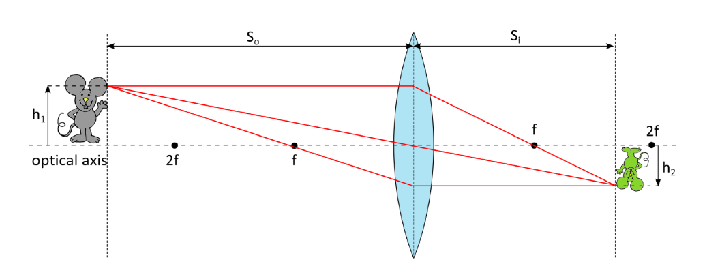
\includegraphics{image_forming_basics.eps}
\caption{Simple image formation using one lens. 
The focal length of the thin lens is $f$, object distance is $s_o$ and image distance is $s_i$. 
The upper ray (parallel to the optical axis on the left) passes through the focal point (denoted as a dot) on the right side of the lens, the middle ray (passing through the centre of the lens) is unrefracted, and the lower ray passes through the focal point on the left side of the lens, and comes out parallel to the optical axis on the other side. 
}
\label{fig:imageforming}
\end{figure}

As the distance between the object and lens ($s_o$) is varied, the distance between the lens and image ($s_i$) also changes. This relationship is determined by the lens foca length ($f$) using the thin lens equation.

\begin{equation}
\frac{1}{s_i}=\frac{1}{s_o}+\frac{1}{f}
\label{eq:thinlens}
\end{equation}

Notice that in Fig.~\ref{fig:imageforming}, the image is smaller than the object. The magnification of a lens is calculated as follows:

\begin{equation}
M = \frac{h_i}{h_o} = -\frac{s_i}{s_o} = \frac{f}{f-s_o}
\label{eq:mag}
\end{equation}

The following conventions are used:
\begin{itemize}
\item $f>0$ for convex lenses
\item $f<0$ for concave lenses
\item $s_o>0$ always
\item $s_i>0$ for real images
\item $s_i<0$ for virtual images
\item Transverse distances above the optical axis are $>0$. Distance
  below are negative. 
\item $M=1$ means unitary magnification (the image is the same size as
  the object). Negative numbers indicated an inverted image.
\end{itemize}

First of all, you should practice drawing ray diagrams by hand. 
You will need to do this later to explain what you observe on the bench.
Make your diagram big, use all of an A4 sheet of paper. 
By convention, the object is is an upright arrow rather than a grey mouse.
Draw the three cardinal rays:
\begin{itemize}
\item The ray parallel to the optical axis goes through $f$ on the image side.
\item The ray that passes through the centre of the lens travels undeflected.
\item Finally, the ray that goes through $f$ on the object side leaves the lens parallel to the optical axis on the image side. 
\end{itemize}


\subsubsection{1. Determine the focal length of a convex lens }
The LED will serve as a light source and an object that can be imaged. 
You will be able to form an image of the LED emitter.
Attach a post holder to a rail carriage and place this on the rail. 
Place the LED in the SM1 holder and attach this to a cage plate and mount this on a post. 
Mount the post to your post-holder and place the LED at one end of the rail.
Power the LED (remembering to use the current-limiting resistor). 
Choose a lens with a focal length of about $f=100~mm$. 
Attach the lens to a lens holder using the lens wrench and a retaining ring (this should already be in the lens holder).
Mount the lens on another carriage and attach to the rail. 
Using a single lens to image an object is known as \textbf{finite conjugate} imaging because the image is paired (i.e. conjugated) with an object at a finite distance from it.
The image plane and sample are \texbf{conjugate planes}.



\begin{itemize}
\item A real image is not formed when the lens is closer then $1f$ to the sample (in this case the LED). 
Place the lens $<1f$ from the LED and use a piece of card on the other side of the lens to verify that no image is formed at any distance from the lens.
Why is no image formed? Hint: what are the rays doing as they come out of the lens? 
\item What happens to the rays at distances greater than $1f$? 
\item Can an image be formed if the lens is $>1f$ from the LED? 
Verify this: place a card very far from the LED (e.g. at $20f$) and slowly move the lens away from the LED. 
What is the distance between the LED and the lens at which you see an image? 
\item Vary the distance between the lens and the LED and measure how far away the image of the LED is formed. 
Fill in the table below. 
Using equation~\ref{eq:thinlens}, calculate $f$ for each value of $s_o$.
\item What is the value of $s_i$ when $s_o=2$?
\end{itemize}

\vspace{2em}
\begin{tabular}{| p{1cm} | p{1cm} | p{1cm} |}
\hline
 $s_o$  &  $s_i$  &  $f$  \\
\hline
\hline
 & & \\ \hline
 & & \\ \hline
 & & \\ \hline
\end{tabular}


\subsubsection{2. Magnifying the image}
As you probably noticed, the size of the image of the LED emitter varied with $s_o$.
A lens produces images of different magnifications depending on $s_o$; an image can always be formed when $s_o>f$. 
To begin thinking about magnification, hand-draw the ray diagram (as in Fig~\ref{fig:imageforming}) for the smallest and largest values of $s_o$ that you used above. 
Note how the angles on the object and image sides of the lens change.
We will now explore how magnification can be explained by the angle at which light comes into focus to form an image. 

\begin{itemize}
\item Place a card in the hard holder and position the $f=100~mm$ lens 100~mm from the card. 
Point the rail out of the window and verify that an image is formed at $1f$. 
\item Repeat with the $f=300~mm$ lens. What do you notice about the image? 
\item Can you draw ray diagrams for these two lenses that explain what you see?
Hint: Light from each point in your distant object arrives as (effectively) parallel rays. 
Light from different regions comes in at different \textit{angles}. 
Try drawing two sets of incoming parallel rays: one that comes in on-axis and one that comes in at an angle. 
It might be easier to do this with the Ray Optics Simulator program.
\item Go back to the lens and LED.
Calculate the values of $s_o$ and $s_i$ which produce $M=-4$ (remember, negative just means inverted) for a $f=100~mm$ lens. 
Measure the size of the LED image and so calculate the size of the LED emitter. 
\item Remember the value of $s_i$ when $s_o=2f$? Therefore what is $M$ when $s_o=2f$?
\end{itemize}

What you have covered above relates to an important property of lenses: that they work the same both forwards and backwards.
Recall the definition of an image-forming condition: \textbf{light rays leaving one point (or region) of the object arrive at some other defined point (or region)}.
This is why no image was formed when the LED was at $s_o=f$, since rays leaving the lens are parallel do not converge on the other side. 
However, you \textit{were} able to form an image at $s_i=f$ when the object was very far away. 
The ray diagrams of these two conditions are \textit{identical}--the only difference is that the object is at $1f$ in the first case and at infinity in the second case.

\subsubsection{3. Virtual images}
At distances $s_o<f$, you were unable to form an image of the sample on the card because the rays emerging from the other side \textit{diverged}.
\begin{itemize}
\item Place the LED $150~mm$ from a $300~mm$ lens. 
\item See how the light diverges coming out of the lens. 
\item Draw the ray diagram for this scenario: Place an object at $f=200~mm$.
Draw the ray that leaves the tip of the object and continues through the middle of the lens. 
Draw the ray that travels parallel to the optical axis and goes through $1f$ on the other side.
See how these rays diverge. 
\end{itemize}

It would seem that no image is formed yet, surprisingly, a \textit{virtual image} is formed on the same side of the lens as the object. 
This may sound like a peculiar concept, but you are already familiar with virtual images as this is how you see images in flat  mirrors (Fig.~/ref{fig:mirror}). 
The extended rays in the case of the mirror can be created from the \textit{diverging} rays from the object. 
In the case of the the lens at $s_o<f$ we also have diverging rays and so can also draw extended rays as we did for the mirror. 
Add the extended rays to your ray diagram. Where do they converge? What does this tell you about the magnification of the virtual image?
\begin{figure}[h]
\center
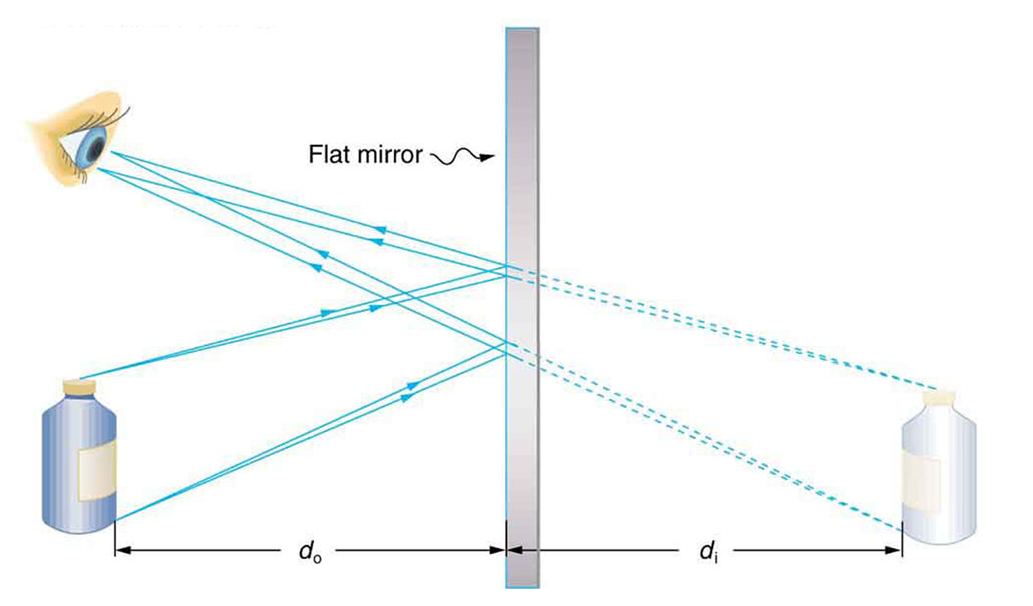
\includegraphics{virtual_image_mirr.eps}
\caption{A virtual image of the bottle is created on the far side of the mirror. 
This is described by the dotted lines which are `extended rays' that are used to form the virtual image. }
\label{fig:mirror}
\end{figure}

A \textbf{real image} is formed on the opposite side of the lens to the sample. 
This allows the detector to be physically separated from the sample, which is rather useful.
As a result, most optical devices use real images. 
A \textbf{virtual image} is formed on the \textit{same} side of the lens as the object. 
Both magnifying glasses and microscope eyepieces use virtual images. 


\clearpage

\subsection{Infinite Conjugate}
You will now explore telescopes and beam expanders.
Beam expanders are critical for building a scanning microscope.
The \textbf{infinite conjugate} refers to the situation where the
object is located at a distance of $1f$ from a lens
(Fig.~\ref{infiniteConjugate}). In this scenario the rays leaving the
lens are parallel and do not converge, so this is not an image forming
condition. Instead, the image can be considered to be infinitely far
away (hence the name). If a second lens is added, then an image can
be formed. The magnification of the image is defined as
(Eq.~\ref{eq:magIC}). 
What useful feature does this arrangement have? 

\begin{equation}
M=-\frac{f_2}{f_1}
\label{eq:magIC}
\end{equation}

\begin{figure}[h]
\center
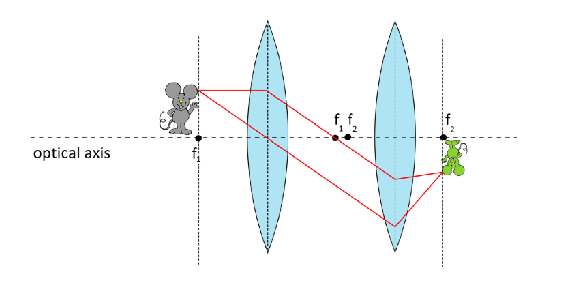
\includegraphics[width=4in]{infiniteConjugate.eps}
\caption{The infinite conjugate.}
\label{infiniteConjugate}
\end{figure}
\subsubsection{A. Building the infinite conjugate}
\begin{itemize}
\item Set up two lenses with different focal lengths on the rail to build the infinite conjugate. 
Place the LED at the $f$ of the first lens and a screen at the $f$ of the second. 
\item Measure the size of the image and calculate the size of the emitter. 
\item Verify the consequences of the infinite space by moving the second lens and keeping the screen at $f$ of the second lens. 
What happens to the image size?
\item Verify Eq.~\ref{eq:magIC} by exploring what happens when lenses of different focal lengths are used. 
\end{itemize}


\subsubsection{B. Building a telescope}
\begin{itemize}
\item Draw an arrow on a coverslip to use as an target to image. 
\item Use a light-guide as a light source with which to illuminate the arrow from behind. 
Use two convex lenses (60~mm and 100~mm, it's up to you which you place nearer the light source and which you place further away). 
\item Put the coverslip at a distance of 150~mm from the first lens, between the lens and the light source. 
Separate the lenses by 250~mm. 
\item Trace the ray diagram. Where will the image be formed? Is the image inverted?  Verify this experimentally. 
\item Move the lenses to alter their relative distance. In which condition is the image virtual? In
which condition real and inverted? In which condition is no image formed?
\end{itemize}


\subsection{Beam expanders}
Lenses can be used to expand the diameter of a light beam, such a laser.
Expanders can be built using either two convex lenses (Fig.~\ref{beamExpander1}) or a convex and concave lens (Fig.~\ref{beamExpander2}). 
In both cases the lenses are set up such that their focal points coincide (i.e. they are separated by the sum of their focal lengths). 
The degree to which a beam is expanded can be calculated as:
\begin{equation}
\frac{d_2}{d_1}=\frac{f_2}{f_1}
\label{eq:beamExp}
\end{equation}

\begin{figure}[h]
\center
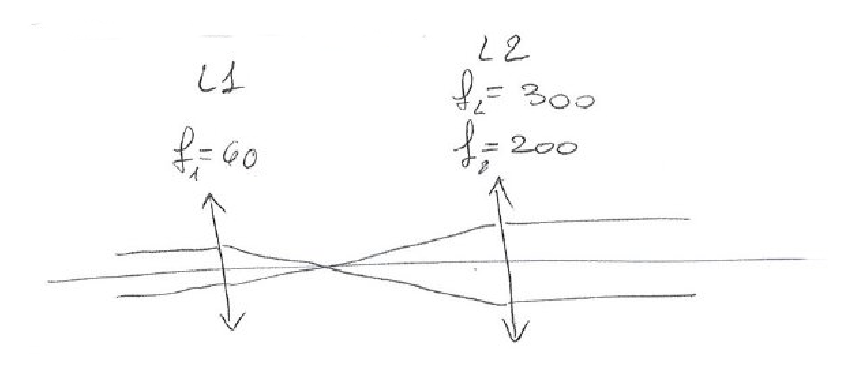
\includegraphics[width=4.5in]{beamExpander1.eps}
\caption{Beam expander with two convex lenses.}
\label{beamExpander1}
\end{figure}

\begin{figure}[h]
\center
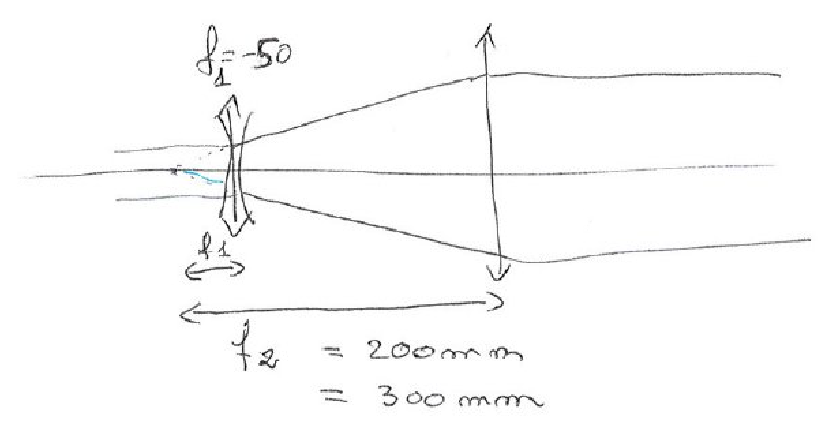
\includegraphics[width=4.5in]{beamExpander2.eps}
\caption{Beam expander with one convex and one concave lens.}
\label{beamExpander2}
\end{figure}

\subsubsection{Aligning the lenses}
You will use a laser as a light source.
The procedure to align the laser and lenses will be explained on the board.

\subsubsection{Experimenting with beam expanders}
\begin{itemize}
\item Construct a beam expander using to convex lenses to expand the beam by at least a factor of three. 
Make sure that the two focal points coincide by checking that the exit beam is collimated
 (i.e. light rays are parallel so beam diameter is constant over long distances). 
\item Measure the size of the expanded beam and so calculate size of the unexpanded beam.
\item Swap out one of the lenses with different convex lens and verify that the expansion factor changes. 
\item What happens if the lenses are closer together or further apart than the sum of their focal lengths?
\item Construct a beam expander using a concave and convex lens. What advantages does this arrangement have?
\end{itemize}

\clearpage

\subsection{Composite optical elements}
Many complex optical elements such as objectives or eyepieces (Fig~\ref{composite}) are built by combining multiple lenses in close proximity. 
In objectives and eyepieces the light doesn't pass through a focal point, as in the telescopes you built. 
The large numbers of optical elements are generally used to correct for optical abberations across the field of view. 
To experiment with composite optical arrangements  you will first construct a beam expander ($f_1$=60~mm lens and a $f_2$=300~mm). 
Light leaving the beam expander will be directed into a composite lens. 
Having the beam expanded will make it easier for you to determine the focal length of the composite elements you will build.

\begin{figure}[h]
\center
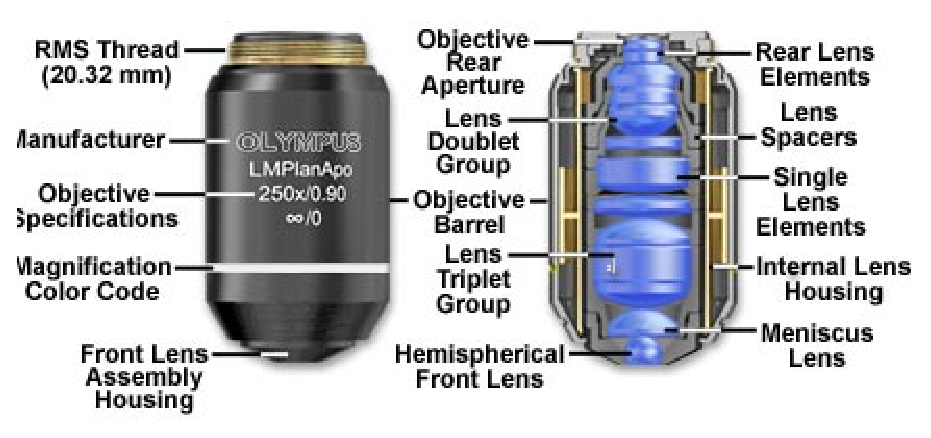
\includegraphics[width=3.5in]{objectivesfigure1.eps}
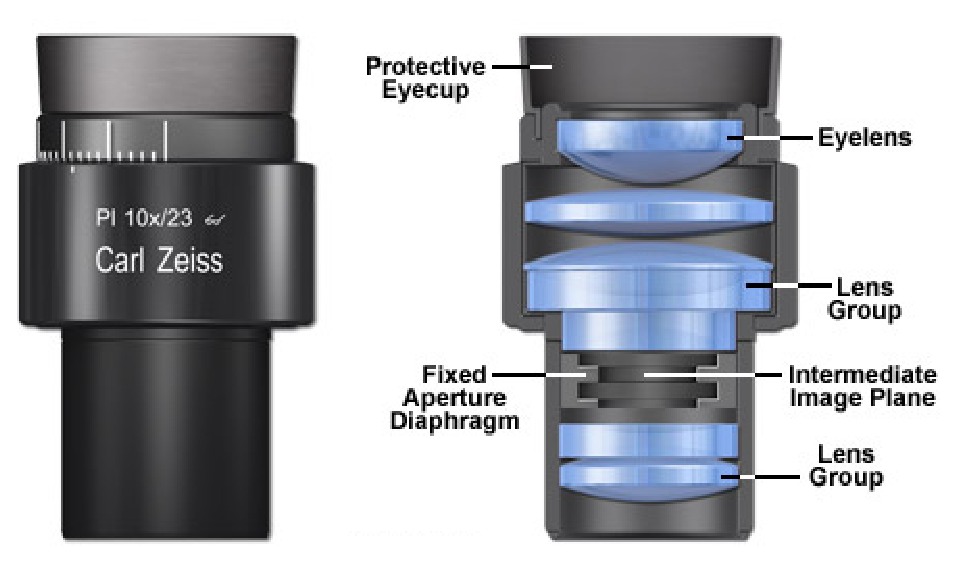
\includegraphics[width=2.8in]{eyepieces5.eps}
\caption{The composite lens arrangements found in microscope
  objectives and eyepieces.}
\label{composite}
\end{figure}

To build a composite optical element simply place a $f$=200~mm lens and a $f$=100~mm adjacent to each other. 
What is the effective focal length of the pair? Verify that it approximates the following:

\begin{equation}
\frac{1}{f}=\frac{1}{f_1}+\frac{1}{f_2}
\label{eq:beamFocalLength}
\end{equation}

\noindent
Swap the $f$=100~mm lens for an $f$=-50~mm lens. Verify that the
combined focal length is shorter.

\subsection{Optics Challenge}
Arrange 4 lenses so as to form a de-magnified, real, upright
image. Hints: 
\begin{itemize}
\item Use one negative lens.
\item Space will be a problem: the lenses will take up the whole rail
  and so you will need to place the target and screen outside of the
  rail. 
\item Use the light-guide to illuminate your target to avoid it
  becoming too dim. 
\item There are multiple solutions to this problem.
\end{itemize}


\clearpage
\section{Illuminating the sample}
Different samples are best illuminated in different ways. In transmission
microscopy the sample is illuminated from the opposite side to which
it is imaged. In fluorescence microscopy (which you will explore later
in the course) the sample is illuminated from the same side, with the
objective serving as the condenser. It is not efficient to illuminate
the sample directly (with no intervening lenses) because light is
emitted in all directions from the source but only a narrow range of
ray angles reach the specimen. In the following two exercises you will
build two different illumination systems: critical and K\"{o}hler. The
exercises will work better if you use a laser to align the lenses
before switching to the LED for imaging the sample. 


\subsection{Critical illumination of a sample}
Critical illumination uses two lenses to focus an image of a light
source onto the specimen (Fig.~\ref{critIlum}). You will now setup
critical illumination on your lens rail. Use an LED as the light
source. Build the condenser using two lenses and place the sample at
their focal point. The lens nearer the LED is known as the
\textbf{collector lens} and the lens nearer the sample is known as the
\textbf{condenser lens}. Use the 30 mm for the collector lens and the
60 mm (convex) for the condenser lens. A suitable sample is a
coverslip with thin lines drawn on with a marker. Place the sample at
the focal point of the condenser lens. Use two more lenses to form an
image of the specimen on a piece of card. The \textbf{objective lens}
($f$=100~mm) follows the specimen, and finally the \textbf{tube lens}
($f$=300~mm) is used to form an image. Set up the lenses and image the
image the sample. What problem do you notice?

Critical illumination can be set up using either a finite or an
infinite conjugate image of the light source. A diaphragm (the
`\textbf{aperture diaphragm}') can be placed between the collector and
condenser lens, at the focal point of the second lens (the condenser
lens) to stop down the range of angles reaching the sample. This
allows the NA of the illuminant to be regulated, providing control
over the resolution, contrast, and depth of field. Add the aperture
diaphragm and observe the effect of regulating the aperture on your
sample image. Does the area illuminated alter when the diaphragm is
closed down?

\begin{figure}[h]
\center
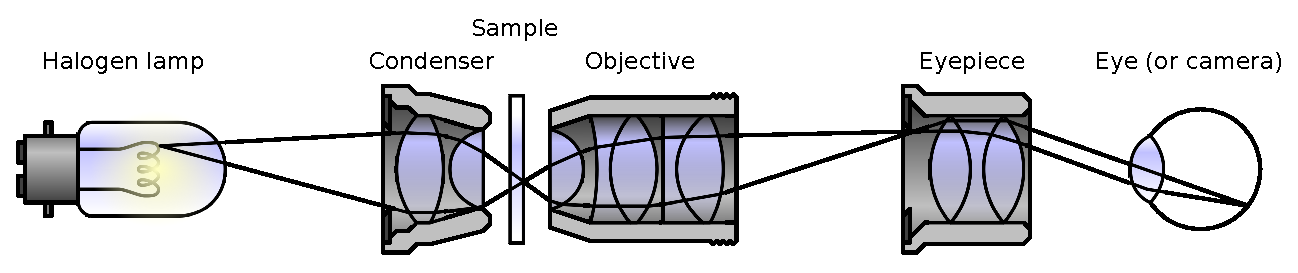
\includegraphics[width=5in]{Critical_Illumination.eps}
\caption{A simple critical illumination set up for visual microscopy.}
\label{critIlum}
\end{figure}


\subsection{K\"{o}hler Illumination}
K\"{o}hler illumination is an important and commonly used technique in
light microscopy, as it provides even illumination of the sample
whilst ensuring the light source (e.g. the bulb filament) is not
visible. This is achieved by adding a third lens (you will use a
$f$=100) so that the image of the filament doesn't appear on the
sample but on the aperture diaphragm (which is the diaphragm located
immediately before the condenser lens). This arrangement not only
permits uniform illumination but also allows a second diaphragm to be
added. This \textbf{field diaphragm} is imaged onto the sample and so
provides a means of regulating the area of illumination. In summary,
whilst an image of the filament is still formed, it occurs at a
different plane to the image formed by the sample. Consequently, when
observing the sample the light source image is out of focus.

You will now convert the critical illumination to K\"{o}hler
illumination.  The components will be arranged in the following order:
\begin{enumerate}
\item Collector lens ($f$=30)
\item Field diaphragm
\item Field lens ($f$=100)
\item Aperture diaphragm
\item Condenser lens ($f$=60)
\item The objective and tube lenses will be as before. 
\end{enumerate}

Again, you will place the LED at one focal length before the collector
lens and the sample at the focal length of the condenser lens. The
arrangement of the components is shown in Fig.~\ref{koehler}. Verify
that you can alter the depth of field by obtaining a second coverslip
and drawing a differet target on it. Stack this alongside the original
sample and vary the sizes of the diaphragms to observe the effects. 


\begin{figure}[h]
\center
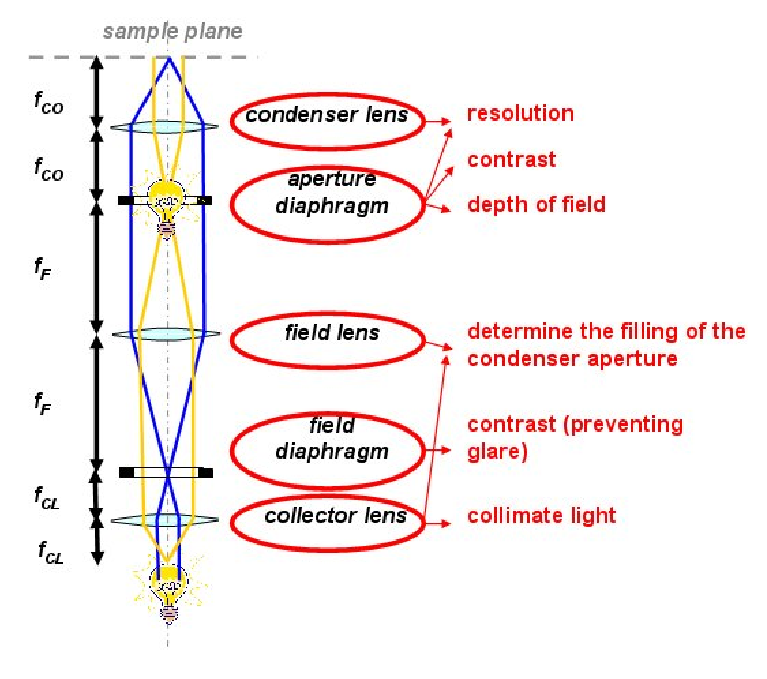
\includegraphics[width=5in]{koehler.eps}
\caption{K\"{o}hler Illumination}
\label{koehler}
\end{figure}




\end{document}
